\documentclass[a4paper,14pt]{extarticle}

\newcommand{\stend}{\textbf{Wb-demo-kit v.2}}

% Путь до папки с общими шаблонами
\newcommand{\pathToCommonFolder}{/home/denilai/Documents/repos/latex/Common}
\newcommand{\pathToScriptsFolder}{/home/denilai/Documents/repos/latex/scripts}
% Название работы в титуле
\newcommand{\workname}{ОТЧЕТ ПО ПРАКТИЧЕСКИМ РАБОТАМ}
% Название дисциплины в титуле
\newcommand{\discipline}{Разработка баз данных}
% Название кафедры в титуле
\newcommand{\kafedra}{Кафедра промышленной информатики (ПИ)}
% Тема работы в титуле
\newcommand{\theme}{Знакомство с оборудованием}
% Должность преподавателя в титуле
\newcommand{\rang}{инженер, ассистент}

% ФИО студента в титуле
\newcommand{\studentfio}{К.~Ю.~Денисов}%\\Д.~Н.~Федосеев\\А.~М.~Сосунов}\\%К.~Ю.~Денисов\\%И.~А.~Кремнев
% ФИО преподавателя в титуле
\newcommand{\teacherfio}{Д.~С.~Киселев}
\newcommand{\signature}{\pathToCommonFolder/denisov-signature}


\usepackage{tabularx}


\usepackage{booktabs}
\newcolumntype{b}{X}
\newcolumntype{s}{>{\hsize=.5\hsize}X}
\newcommand{\heading}[1]{\multicolumn{1}{c}{#1}}

% установка размера шрифта для всего документа
%\fontsize{20pt}{18pt}\selectfont
\usepackage{extsizes} % Возможность сделать 14-й шрифт

% Вставка заготовки преамбулы
% Этот шаблон документа разработан в 2014 году
% Данилом Фёдоровых (danil@fedorovykh.ru) 
% для использования в курсе 
% <<Документы и презентации в \LaTeX>>, записанном НИУ ВШЭ
% для Coursera.org: http://coursera.org/course/latex .
% Исходная версия шаблона --- 
% https://www.writelatex.com/coursera/latex/5.3

% В этом документе преамбула

% Для корректного использования русских символов в формулах
% пакеты hyperref и настройки, связанные с ним, стоит загуржать
% перед загрузкой пакета mathtext



% поддержка русских букв
% кодировка шрифта
%\usepackage[T2A]{fontenc} 
\usepackage{pscyr}

% использование ненумеровонного абзаца с добавлением его в содержаниеl

\newcommand{\anonsection}[1]{\section*{#1}\addcontentsline{toc}{section}{#1}}
\newcommand{\sectionunderl}[1]{\section*{\underline{#1}}}


% настройка окружения enumerate
\usepackage{enumitem}
\setlist{noitemsep}
\setlist[enumerate]{labelsep=*, leftmargin=1.5pc}

\usepackage{hyperref}

% сначала ставить \usepackage{extsizes} % Возможность сделать 14-й шрифт
% для корректной установки полей вставлять преамбулу следует в последнюю очередь (но перед дерективой замены \rmdefault)
\usepackage[top=20mm,bottom=25mm,left=35mm,right=20mm]{geometry} % Простой способ задавать поля

\hypersetup{				% Гиперссылки
	unicode=true,           % русские буквы в раздела PDF
	pdftitle={Заголовок},   % Заголовок
	pdfauthor={Автор},      % Автор
	pdfsubject={Тема},      % Тема
	pdfcreator={Создатель}, % Создатель
	pdfproducer={Производитель}, % Производитель
	pdfkeywords={keyword1} {key2} {key3}, % Ключевые слова
	colorlinks=true,       	% false: ссылки в рамках; true: цветные ссылки
	linkcolor=red,          % внутренние ссылки
	citecolor=black,        % на библиографию
	filecolor=magenta,      % на файлы
	urlcolor=blue           % на URL
}

%%% Работа с русским языком
\usepackage{cmap}					% поиск в PDF
\usepackage{mathtext} 				% русские буквы в формулах
\usepackage[T2A]{fontenc}			% кодировка
\usepackage[utf8]{inputenc}			% кодировка исходного текста
\usepackage[english,russian]{babel}	% локализация и переносы
\usepackage{indentfirst}
\frenchspacing

%для изменения названия списка иллюстраций
\usepackage{tocloft}


\renewcommand{\epsilon}{\ensuremath{\varepsilon}}
\renewcommand{\phi}{\ensuremath{\varphi}}
\renewcommand{\kappa}{\ensuremath{\varkappa}}
\renewcommand{\le}{\ensuremath{\leqslant}}
\renewcommand{\leq}{\ensuremath{\leqslant}}
\renewcommand{\ge}{\ensuremath{\geqslant}}
\renewcommand{\geq}{\ensuremath{\geqslant}}
\renewcommand{\emptyset}{\varnothing}

% Изменения параметров списка иллюстраций
\renewcommand{\cftfigfont}{Рисунок } % добавляем везде "Рисунок" перед номером
\addto\captionsrussian{\renewcommand\listfigurename{Список иллюстративного материала}}

\newcommand{\tm}{\texttrademark\ }
\newcommand{\reg}{\textregistered\ }


%%% Дополнительная работа с математикой
\usepackage{amsmath,amsfonts,amssymb,amsthm,mathtools} % AMS
\usepackage{icomma} % "Умная" запятая: $0,2$ --- число, $0, 2$ --- перечисление

%% Номера формул
%\mathtoolsset{showonlyrefs=true} % Показывать номера только у тех формул, на которые есть \eqref{} в тексте.
%\usepackage{leqno} % Нумереация формул слева

%% Свои команды
\DeclareMathOperator{\sgn}{\mathop{sgn}}

%% Перенос знаков в формулах (по Львовскому)
\newcommand*{\hm}[1]{#1\nobreak\discretionary{}
{\hbox{$\mathsurround=0pt #1$}}{}}


% отступ для первого абзаца главы или параграфа
%\usepackage{indentfirst}

%%% Работа с картинками
\usepackage{graphicx}  % Для вставки рисунков
\graphicspath{{images/}{screnshots/}}  % папки с картинками
\DeclareGraphicsExtensions{.pdf,.png,.jpg}
\setlength\fboxsep{3pt} % Отступ рамки \fbox{} от рисунка
\setlength\fboxrule{1pt} % Толщина линий рамки \fbox{}
\usepackage{wrapfig} % Обтекание рисунков текстом

%%% Работа с таблицами
\usepackage{array,tabularx,tabulary,booktabs} % Дополнительная работа с таблицами
\usepackage{longtable}  % Длинные таблицы
\usepackage{multirow} % Слияние строк в таблице

%%% Теоремы
\theoremstyle{plain} % Это стиль по умолчанию, его можно не переопределять.
\newtheorem{theorem}{Теорема}[section]
\newtheorem{proposition}[theorem]{Утверждение}

\theoremstyle{plain} % Это стиль по умолчанию, его можно не переопределять.
\newtheorem{work}{Практическая работа}[part]


 
 
\theoremstyle{definition} % "Определение"
\newtheorem{corollary}{Следствие}[theorem]
\newtheorem{problem}{Задача}[section]
 
\theoremstyle{remark} % "Примечание"
\newtheorem*{nonum}{Решение}



%%% Программирование
\usepackage{etoolbox} % логические операторы

%%% Страница

%	\usepackage{fancyhdr} % Колонтитулы
% 	\pagestyle{fancy}
%   \renewcommand{\headrulewidth}{0pt}  % Толщина линейки, отчеркивающей верхний колонтитул
% 	\lfoot{Нижний левый}
% 	\rfoot{Нижний правый}
% 	\rhead{Верхний правый}
% 	\chead{Верхний в центре}
% 	\lhead{Верхний левый}
%	\cfoot{Нижний в центре} % По умолчанию здесь номер страницы

\usepackage{setspace} % Интерлиньяж
\onehalfspacing % Интерлиньяж 1.5
%\doublespacing % Интерлиньяж 2
%\singlespacing % Интерлиньяж 1

\usepackage{lastpage} % Узнать, сколько всего страниц в документе.

\usepackage{soul} % Модификаторы начертания


\usepackage[usenames,dvipsnames,svgnames,table,rgb]{xcolor}


\usepackage{csquotes} % Еще инструменты для ссылок

%\usepackage[style=authoryear,maxcitenames=2,backend=biber,sorting=nty]{biblatex}

\usepackage{multicol} % Несколько колонок

\usepackage{tikz} % Работа с графикой
\usepackage{pgfplots}
\usepackage{pgfplotstable}

% модуль для вставки рыбы
\usepackage{blindtext}

\usepackage{listings}
\usepackage{color}


% для поворота отдельной страницы. Использовать окружение \landscape
\usepackage{pdflscape} 
\usepackage{rotating} 


\definecolor{mygreen}{rgb}{0,0.6,0}
\definecolor{mygray}{rgb}{0.5,0.5,0.5}
\definecolor{mymauve}{rgb}{0.58,0,0.82}


% пример импорта файла
%\lstinputlisting{/home/denilai/repomy/conf/distributions}

\lstset{
	language=Python,
	basicstyle=\footnotesize,        % the size of the fonts that are used for the code
	numbers=left,                    % where to put the line-numbers; possible values are (none, left, right)
	numbersep=5pt,                   % how far the line-numbers are from the code
	numberstyle=\tiny\color{mygray}, % the style that is used for the line-numbers
	stepnumber=2,                    % the step between two line-numbers. If it's 1, each line will be numbered
	% Tab - 2 пробела
	tabsize=2,    
	% Автоматический перенос строк
	breaklines=true,
	frame=single,
	breakatwhitespace=true,
	title=\lstname 
}



\author{Кирилл Денисов}
\title{Лабораторная работа №1}
\date{\today}

\renewcommand{\withouttheme}{1}

\newcommand{\erassistant}{\texttt{ErAssistant}}
\newcommand{\erdatamodaler}{\texttt{ERwin Data Modeler}}
\newcommand{\methodsection}{Работа по методическим указаниям}
\newcommand{\individual}{Индивидуальный вариант}

%если нужна тема работы в отчете, то указать в скобках что-либо, иначе оаставить пустым
%\renewcommand{\withouttheme}{}
%если нужна дата представления отчета, то указать в скобках что-либо
%\renewcommand{\withoutsubmissiondate}{1}

% установка полуторного интервала
% \usepackage{setspace}  
% \onehalfspacing

% использовать Times New Roman
\renewcommand{\rmdefault}{ftm}


\begin{document}
	
	\gdef\capnames{
		\gdef\figurename{Рисунок}
		\gdef\chaptername{ГЛАВА}
		\gdef\appendixname{ПРИЛОЖЕНИЕ}
		\gdef\bibname{СПИСОК ЛИТЕРАТУРЫ}
		\gdef\contentsname{СОДЕРЖАНИЕ}
		\bibliographystyle{gost71s}
	}
	
	
	\thispagestyle{empty}
	% Вставка первого титульного листа
	% Есть две версии титульного листа - одиночный (titul) и групповой (titulAll)
	%\newcommand{\withouttheme}{} добавить эту переменную для определения, нужна ли тема
%     {} - нужна
%    {1} - не нужна

%\newcommand{\withoutsubmissiondate}{} добавить эту переменную для определения, нужен ли срок предоставления отчета
%     {} - нужен
%    {1} - не нужен
\begin{center}
	\begin{figure}[h!]
		\begin{center}
		
\includegraphics[width=0.17\linewidth]{\pathToCommonFolder/gerb}
		%\caption{}\label{pic:first}
		%	\vspace{5ex}
		\end{center}	
	\end{figure}
 	\small	МИНОБРНАУКИ РОССИИ \\
	Федеральное государственное бюджетное образовательное учреждение\\
						высшего профессионального образования\\
\normalsize					
\textbf{«МИРЭА – Российский технологический университет»\\
						РТУ МИРЭА}\\
						\noindent\rule{1\linewidth}{1pt}\\
       Институт информационных технологий\\ %\vspace{2ex}
					\kafedra\\
		\vspace{3ex}
			\large \textbf{\workname}  \\
		%\vspace{1ex}
						по дисциплине\\ «\discipline» \\
		\vspace{3ex}
		\if \withouttheme
			\textbf{Тема работы:}\\ <<\theme>>
		\fi
\vspace{3ex}
\small
\begin{table}[h!]
\begin{tabular}{p{0.14\linewidth}p{0.38\linewidth}p{0.25\linewidth}p{0.2\linewidth}}
	\textbf{Выполнил:} & студент группы ИВБО-02-19 & \studentfio &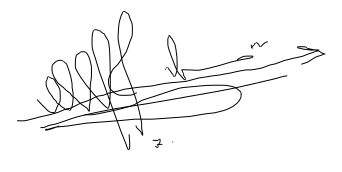
\includegraphics[width=0.8\linewidth]{\signature}\\ \\
	\textbf{Принял:} & \rang & \teacherfio 
\end{tabular}
\end{table}
\end{center}

\begin{flushleft}
	\begin{tabular}{p{0.25\linewidth}l}

		Работа выполена & <<\noindent\rule{2em}{1pt}>>
		                    \noindent\rule{5em}{1pt} 202\noindent\rule{1em}{1pt} \\

		<<Зачтено>> & <<\noindent\rule{2em}{1pt}>>
		\noindent\rule{5em}{1pt} 202\noindent\rule{1em}{1pt} \\

	\end{tabular}
\end{flushleft}

\normalsize
\begin{center}	
\vfill 
Москва 2021
\end{center}

	\newpage
	\tableofcontents
	\newpage
	%\listoftables

\normalsize

\section{Построение модели данных}
\subsection{\methodsection}
\subsubsection*{Описание предметной области}
Компания занимается производством и продажей небольших статуэток,
раскрашиваемых вручную. Компания имеет несколько производственных
направлений. Миниатюры изготавливаются из гипса, олова или алюминия.

Компания распространяет свои товары по трем каналам. Компания содержит
пять собственных розничных магазинов. Помимо этого, компания владеет
сайтом, на котором ведется online-торговля, и осуществляет оптовые поставки
сторонним
дистрибьюторам.
Для
анализа
статистики,
системой автоматизации производства, нужен интерактивный аналитический
инструмент. Поэтому необходимо спроектировать и построить модель данных,
которая станет хранилищем информации по производству.

В ходе производства изделий система автоматизации производства
управляет всеми станками компании. Каждый станок реализует полный цикл
производства изделий, включая:
\begin{itemize}
	\item заполнение формы сырьем (гипсом, оловом или алюминием);
	\item затвердевание материала;
	\item  удаление изделия из формы после затвердевания;
	\item при необходимости автоматизированная раскраска изделий (оловянные фигурки не раскрашиваются);
	\item сушку после покраски (при необходимости).
\end{itemize}


Покраска и сушка могут производиться за несколько этапов в зависимости
от сложности изделия. По мере готовности изделия проходят проверку,
выполняемую оператором станка.

Оператор станка регистрируется в системе. В ходе этого процесса оператор
сообщает системе автоматизации производства тип производимых изделии и
объем загруженного в машину сырья. Оператор также делает в системе запись
при отбраковке изделий.

В ходе
интервью необходимые для эффективного анализа статистики:
\begin{itemize}

\item  число принятых изделий по объему сырья, видам изделий, машинам и
\item  время формовки и затвердевания по видам изделий, машинам и дням;
\item  время покраски и сушки по типам краски, видам изделий, машинам и
\item  сворачивание по подтипам изделий, которые сворачиваются по типам;
\item  сворачивание по типам машин, которые сворачиваются по материалам
(гипс, олово или алюминий);
\item  сворачивание машин по фабрикам, которые сворачиваются по странам;
\item  сворачивание дней по месяцам, месяцев — по кварталам, кварталов – по
\item  возможность фильтрации информации по производителю и дате
\end{itemize}
покупки машины.
Анализ файла-экспорта из системы автоматизации производства показал,
что для каждого вида производимых изделий есть отдельная строка, в которой
присутствует следующая информация:
\begin{itemize}
	\item  тип изделия;
	\item  объем сырья;
	\item  номер машины;
	\item  личный номер оператора;
	\item  время и дата начала производства (когда серия начата);
	\item  время и дата окончания производства (когда серия закончена);
	\item  флаг отбраковки.
\end{itemize}
\subsubsection*{Построение модели}
По приведенному описанию предметной области построим ее модель в среде \erassistant. Укажем линии связей, назначим им имена, укажем типы и кратность связей. В результате работы, модель примет вид, приведенный на Рисунке \ref{fig:1-metod}.

% TODO: \usepackage{graphicx} required
\begin{figure}[h!]
	\centering
	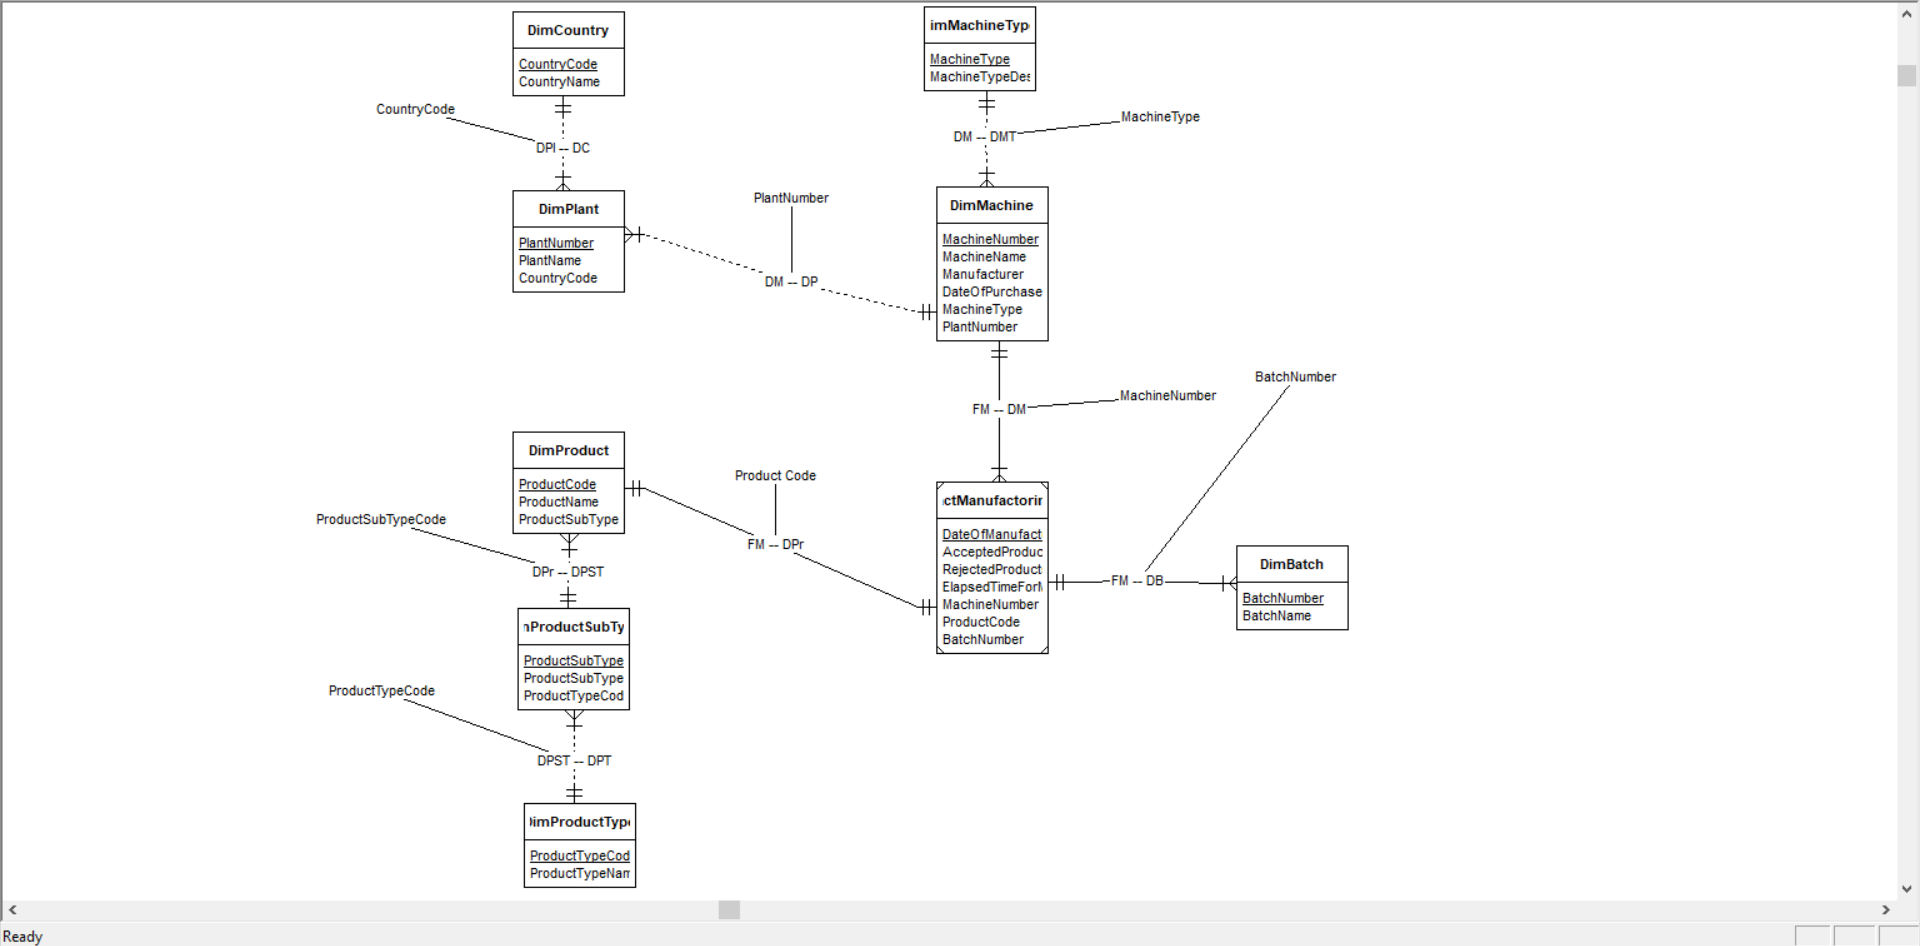
\includegraphics[width=0.7\linewidth]{images/1-metod}
	\caption{Модель данных Производства со связями}
	\label{fig:1-metod}
\end{figure}
%Сформируем отчет по данной модели средствами \erassistant. Перед формированием отчета убедимся в отсутствии ошибок в построенной модели. Проверка наличия ошибок осуществляется нажатием кнопки "Check~Diagram" на панели инструментов в верхней части экрана (см. рисунки \ref{fig:1-report}, \ref{fig:1-report2}).


%% TODO: \usepackage{graphicx} required
%\begin{figure}[h!]
%	\centering
%	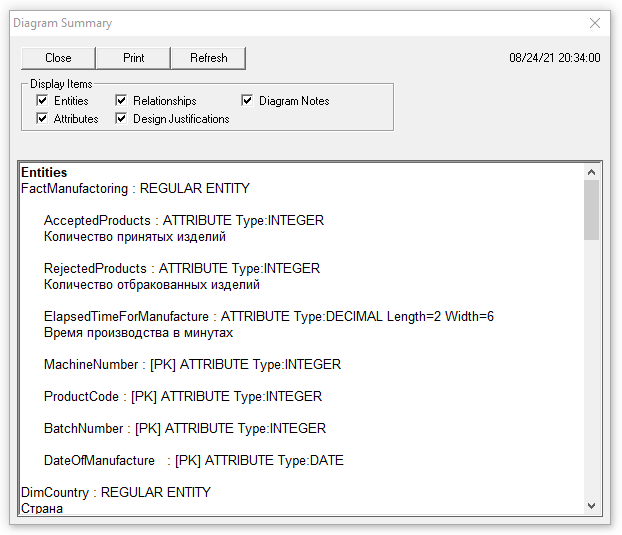
\includegraphics[width=0.7\linewidth]{images/1-report}
%	\caption{Отчет разработанной модели данных производства часть 1}
%	\label{fig:1-report}
%\end{figure}
%
%% TODO: \usepackage{graphicx} required
%\begin{figure}[h!]
%	\centering
%	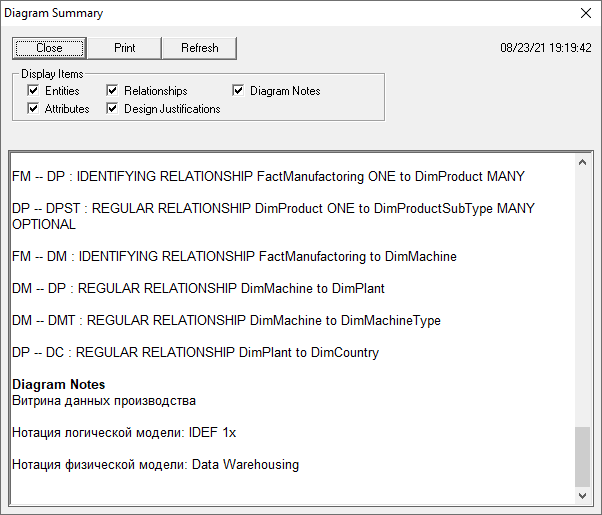
\includegraphics[width=0.7\linewidth]{images/1-report2}
%	\caption{Отчет разработанной модели данных производства часть 2}
%	\label{fig:1-report2}
%\end{figure}

%Отчет по построенной модели приведен на Рисунке ... .
\newpage
\subsection{\individual}
\subsubsection*{Описание предметной области}
В качестве индивидуального задания была выбрана реализация модели информационной системы по хранению и анализу данных  предприятия, занимающегося сборкой и поставкой спортивных велосипедов для конечных потребителей по индивидуальному заказу.

Предприятие располагает широким выборов компонентов и комплектующих для сборки велосипедов следующих типов:
\begin{itemize}
	\item Дорожный;
	\item Горный;
	\item Кросс-кантри;
	\item Эндуро;
	\item Прогулочный.
\end{itemize}

Предприятие может предложить сконфигурировать сборку велосипеда, отдельно выбрав каждый из предложенных компонентов:
\begin{itemize}
	\item Рама;
	\item Вилка;
	\item Руль;
	\item Трансмиссия;
	\item Колеса;
	\item Тормозная система.
\end{itemize}

Контроль над выполнением работ по сборке велосипеда проводится в виде учета всех операций по сборке, настройке и тестированию, проводимых на территории предприятия ее сотрудниками. При этом в каждой записи содержится следующая информация о проведенных работах:
\begin{enumerate}
	\item Внутренний номер изделия;
	\item Время;
	\item Этап работ;
	\item Название цеха;
	\item Имя мастера;
	\item Статус;
	\item Примечание.
\end{enumerate}

На предприятии ведется учет всех компонентов велосипедов.
В базе данных предприятия хранится информация о каждом компоненте, приобретенном у партнеров или изготовленном самостоятельно. В независимости от типа компонента он обладает общей информацией о наименовании производителя, месте и времени изготовления, типе и рекомендованной розничной цене. 

Также каждый компонент имеет особые сведения, присущие данному типу детали.

\subsubsection*{Построение модели}
После приведения общих сведений о роде деятельности предприятия, факторизируем модель данных информационной системы предприятия в среде \erassistant. См. Рисунок \ref{fig:1-cycle}.
% TODO: \usepackage{graphicx} required
\begin{figure}[hpbt]
	\centering
	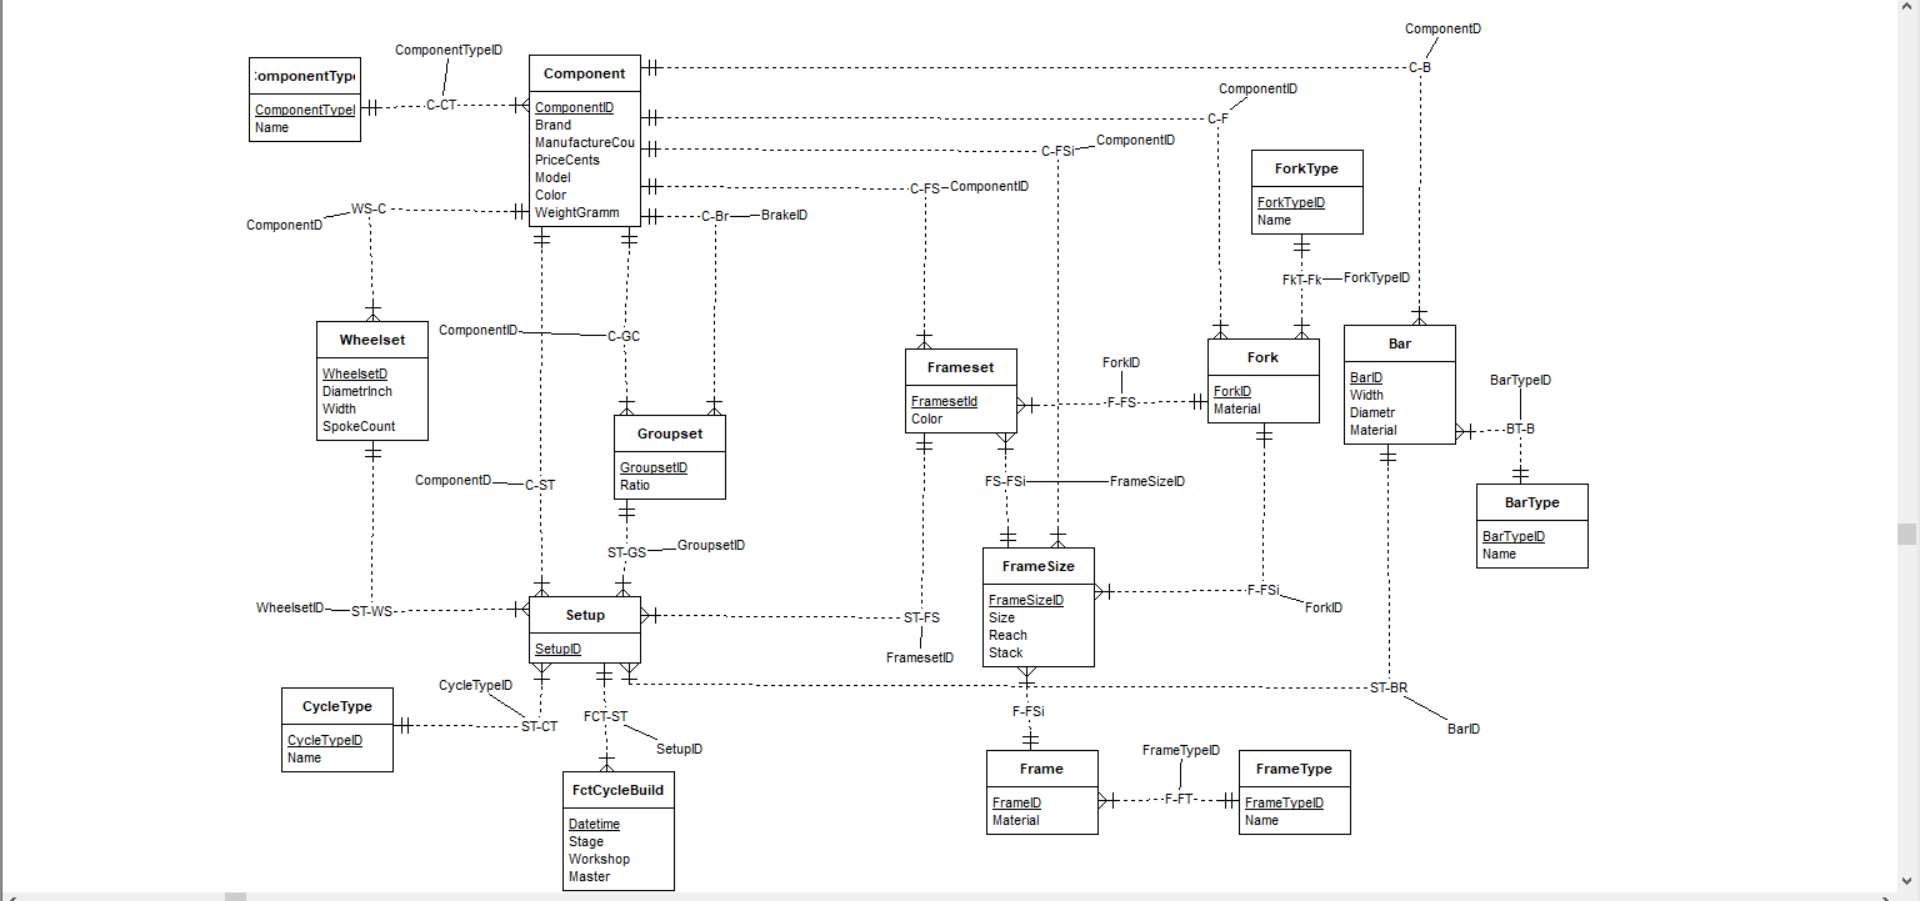
\includegraphics[width=1\linewidth]{images/1-cycle}
	\caption{Модель данных вело-предприятия}
	\label{fig:1-cycle}
\end{figure}

Укажем названия связей, их идентификаторы и кратность, исходя из вида отношений, выстроенных между сущностями.

На данном этапе выполнения работы мы реализовали модель данных будущего хранилища данных, планируемого к применению в компании, занимающейся сборкой и поставкой велосипедов по индивидуальному заказу.

\section{Создание логической\\и физической модели данных}
\subsection{\methodsection}
\subsection*{Теоретический материал}
На этапе \texttt{инфологического} проектирования базы данных должна быть построена
модель предметной области, не привязанная к конкретной СУБД, понятная не только
разработчикам информационной системы, но и экономистам, менеджерам и другим
специалистам. В то же время модель предметной области должна максимально точно
отражать семантику предметной области и позволять легко перейти к модели данных
конкретной СУБД.

Такими моделями являются модели <<сущность-связь>>. Известно несколько
методологий построения моделей <<сущность-связь>>. Наибольшее распространение
получила методология IDEF1X. Рассмотрим построение моделей "сущность-связь",
ориентируясь на продукт CA ERwin Data Modeler. ERwin имеет два уровня
представления модели:

\textbf{Логический уровень} --- это уровень, соответствующий \texttt{инфологическому} этапу проектирования
и не привязанный к конкретной СУБД. Модели логического уровня оперируют с
понятиями сущностей, атрибутов и связей, которые на этом уровне именуются на
естественном языке (в нашем случае – на русском) так, как они называются в
реальном мире.

\textbf{Физический уровень} --- это отображение логической модели на модель данных
конкретной СУБД. Одной логической модели может соответствовать несколько
физических моделей. Причем, Erwin (как и другие CASE-системы проектирования баз
данных) позволяет автоматизировать отображение логической модели на физическую.

Модель <<сущность-связь>> строится в виде диаграммы <<сущность-связь>>,
основными компонентами которой являются сущности (Entity) и связи\\(Relationship).
Отсюда происходят часто используемые названия модели (ER-модель) и диаграммы
(ER-диаграмма).

В ходе данной практической работы нами была описана и построена логическая и физическая модель данных средствами ПО \erdatamodaler.

Порядок построения модели данных в среде ERwin рассмотрим на примере
автоматизированной информационной системы "Реализация средств вычислительной
техники", предназначенной для учета продаж настольных компьютеров по заказам
клиентов.

Создание модели данных начинается с разработки логической модели, которая
должна представлять состав сущностей предметной области с перечнем атрибутов и
отношений между ними.

%В зависимости от глубины представления информации о данных различают 3
%подуровня логического уровня модели данных:
%\begin{itemize}
%	\item  диаграмма сущность – связь \texttt{(Entity Relationship Diagram, ERD)};
%	\item модель данных, основанная на ключах (\texttt{Key Based model, KB)}; --- полная атрибутивная модель данных \texttt{(Fully Attributed model, FA)}.
%\end{itemize}
%
%\texttt{Диаграмма сущность-связь} включает сущности и взаимосвязи, отражающие
%основные бизнес-правила предметной области.
%
%\texttt{Модель данных, основанная на ключах} --- более подробное представление данных.
%Данная модель включает описание всех сущностей и первичных ключей,
%необходимых для подробного описания предметной области.
%
%\texttt{Полная атрибутивная модель данных} --- наиболее детальное представление
%структуры данных предметной области. Данная модель представляет данные в третьей
%нормальной форме и включает все сущности, атрибуты и связи.
%
%Логическим соотношением между сущностями является \textbf{связь}. Каждому виду
%связи соответствует определенная кнопка, расположенная на палитре инструментов.
%Имя связи выражает некоторое ограничение или правило и облегчает чтение
%диаграммы. Каждая связь должна именоваться глаголом или глагольной фразой.

Результат разработки логической модели данных системы <<Реализация средств
вычислительной техники>>, предназначенной для учета продаж настольных
компьютеров по заказам клиентов приведен на Рисунке \ref{fig:2-logical-model-method}.

% TODO: \usepackage{graphicx} required
\begin{figure}[htpb]
	\centering
	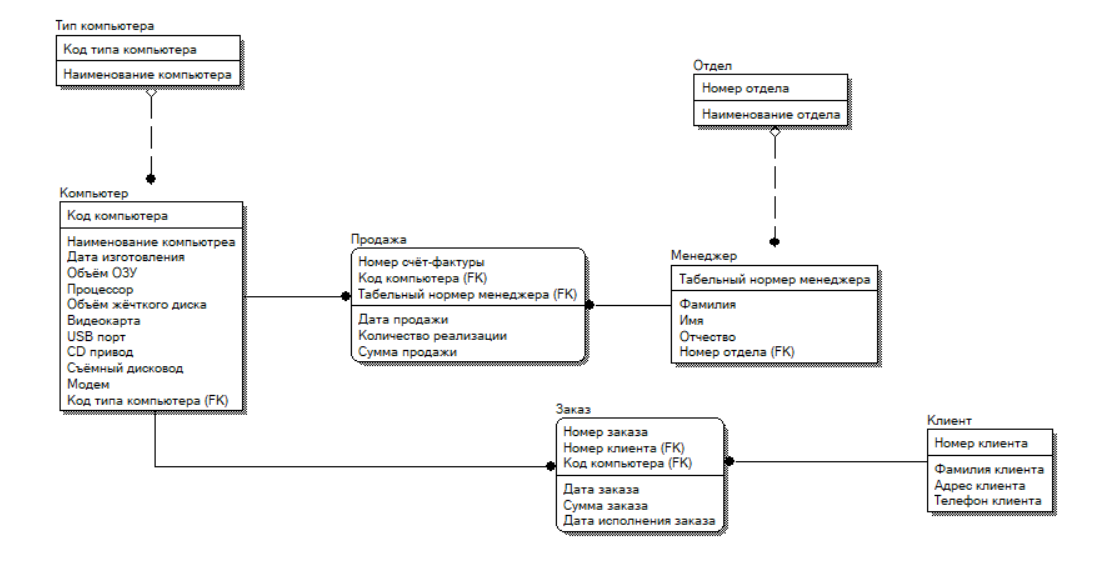
\includegraphics[width=0.7\linewidth]{images/2-method}
	\caption{Логическая модель данных системы <<Реализация средств вычислительной техники>>}
	\label{fig:2-logical-model-method}
\end{figure}

Для построения физической модели данных системы, следует определиться с СУБД, в которой будет реализована модель. При построении физической модели данных следует учитывать формальную теория представления и обработки данных в конкретной системе управления базами данных (СУБД).

В данной практической работе в качестве СУБД выбрана MySQL.

Приступим к построению физической модели данных системы <<Реализация средств вычислительной техники>>. Результат работы можно видеть на рисунке \ref{fig:2-phisical-model}.

% TODO: \usepackage{graphicx} required
\begin{figure}[h!]
	\centering
	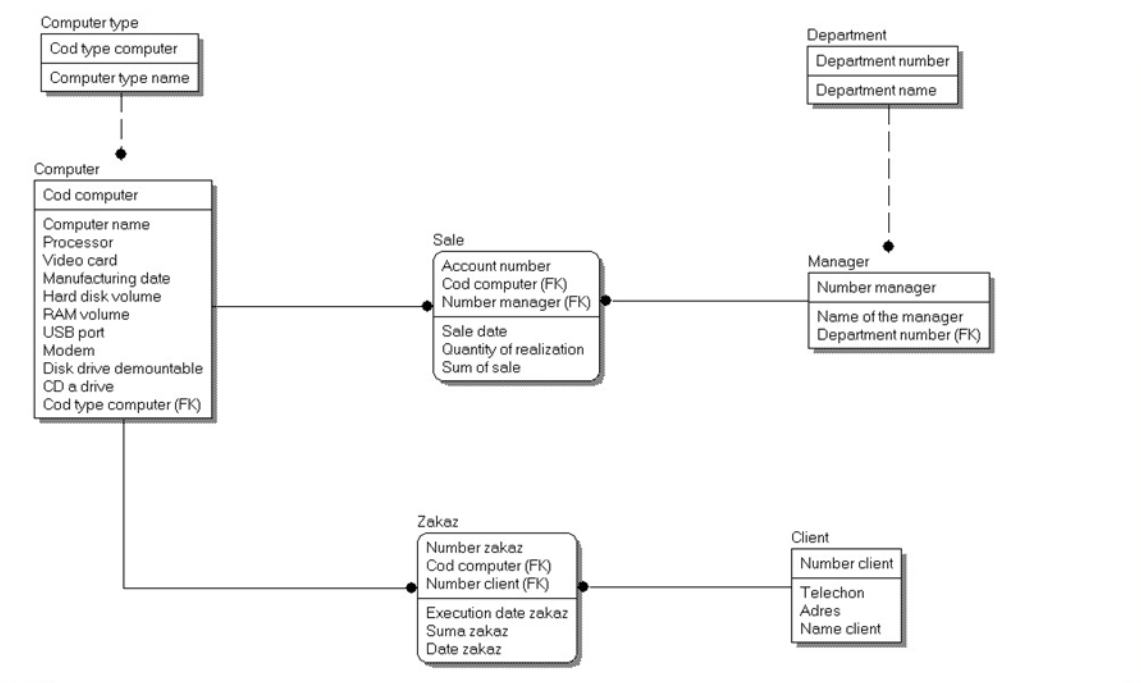
\includegraphics[width=0.7\linewidth]{images/2-phisical-model}
	\caption{Физическая модель данных системы <<Реализация средств вычислительной техники>>}
	\label{fig:2-phisical-model}
\end{figure}

\section{\individual}
Приступим к построению логической модели данных системы <<Велосипедное предприятие>>. 
В соответствии с моделью, реализованной в ходе первой практической работы, добавим в рабочую область следующие сущности:
\begin{itemize}
	\item Component;
	\item FrameInfo;
	\item Frame;
	\item Frameset;
	\item FrameSize;
	\item Fork;
	\item ComponentType;
	\item Wheelset;
	\item Groupset;
	\item Brake;
	\item FctCycleBuild;
	\item CycleType;
	\item Bar;
	\item Setup.
\end{itemize}
Добавим связи между сущностями в соответствии с ранее построенной моделью. Логическая модель системы <<Велосипедное предприятие>> приведена на рисунке \ref{fig:2-cycle-logical}.

% TODO: \usepackage{graphicx} required
\begin{figure}[h!]
	\centering
	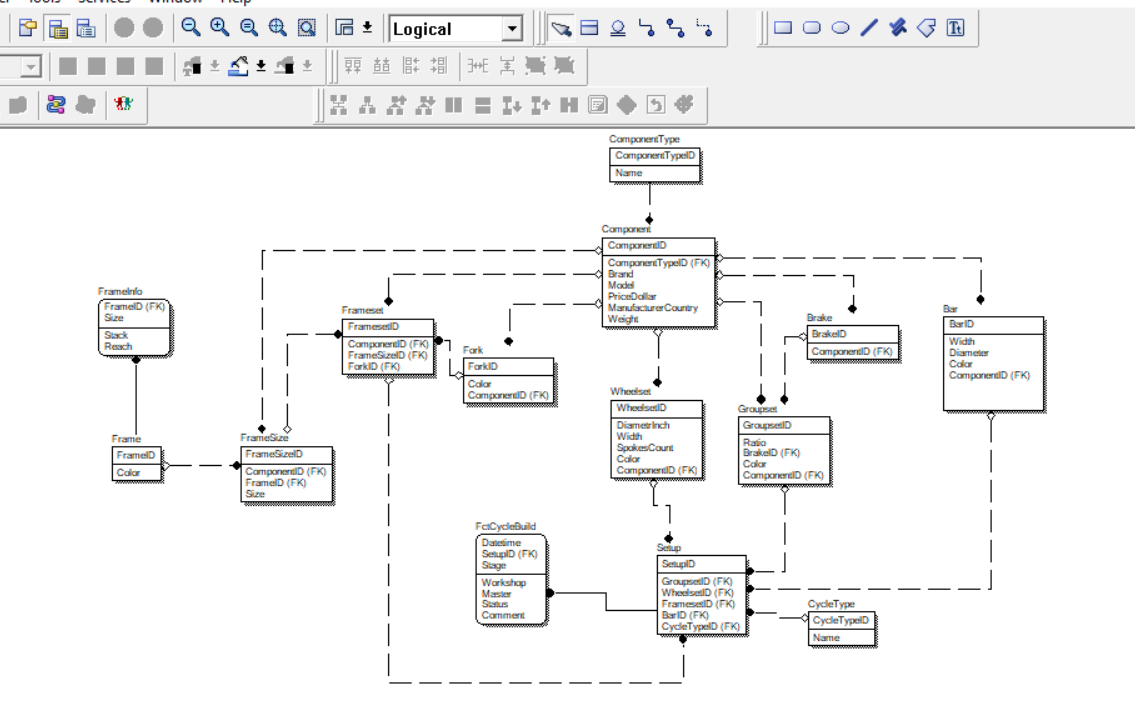
\includegraphics[width=0.8\linewidth]{images/2-cycle-logical}
	\caption{Логическая модель данных системы <<Велосипедное предприятие>>}
	\label{fig:2-cycle-logical}
\end{figure}

После уточнения типов данных, выбранных в соответствии с предметной областью и спецификой СУБД MySQL, построим физическую модель данных (см. рисунок \ref{fig:2-cycle-phisical}).

% TODO: \usepackage{graphicx} required
\begin{figure}[h!]
	\centering
	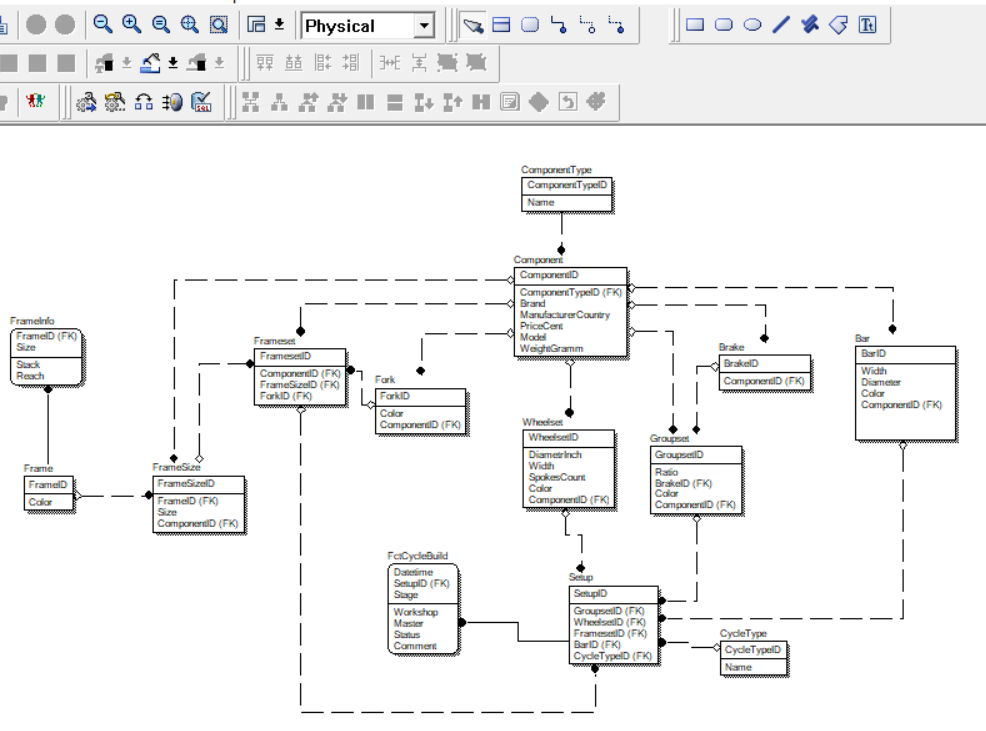
\includegraphics[width=0.8\linewidth]{images/2-cycle-phisical}
	\caption{Физическая модель данных системы <<Велосипедное предприятие>>}
	\label{fig:2-cycle-phisical}
\end{figure}

После реализации физической и логической модели можно приступать к реализации модели данной системы в СУБД MySQL.


\section{Создание базы данных}
\subsection{\methodsection}
В ходе данной практической работы была создана база данных \texttt{forum}, которая хранит в себе сведения о пользователях форума и размещенных ими темах.

Помимо суперпользователя root, был создан пользователь denilai, под которым производятся все манипуляции с данными.

Создадим базу данных \texttt{forum} с помощью команды \texttt{create database forum;}


Создадим таблицу \texttt{users} с помощью данных команд (см. рисунок \ref{fig:create-users}):

% TODO: \usepackage{graphicx} required
\begin{figure}[h!]
	\centering
	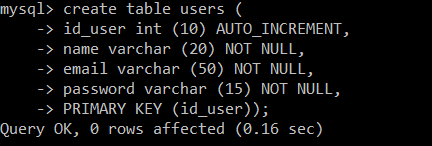
\includegraphics[width=0.6\linewidth]{images/create-users}
	\caption{}
	\label{fig:create-users}
\end{figure}

%\begin{lstlisting}
%create table users (
%	id_user int (10) AUTO_INCREMENT,
%	name varchar(20) NOT NULL,
%	email varchar(50) NOT NULL,
%	password varchar(15) NOT NULL,
%	PRIMARY KEY (id_user)
%);
%\end{lstlisting}

Создадим таблицу \texttt{topics} с помощью данных команд (см. рисунок \ref{fig:create-topics}):

% TODO: \usepackage{graphicx} required
\begin{figure}[h!]
	\centering
	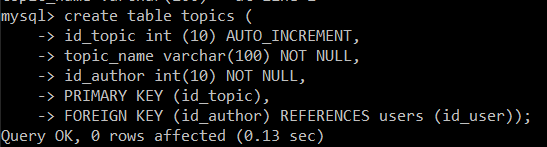
\includegraphics[width=0.6\linewidth]{images/create-topics}
	\caption{}
	\label{fig:create-topics}
\end{figure}

%\begin{lstlisting}
%create table topics (
%	id_topic int (10) AUTO_INCREMENT,
%	topic_name varchar(100) NOT NULL,
%	id_author int (10) NOT NULL,
%	PRIMARY KEY (id_topic),
%	FOREIGN KEY (id_author) REFERENCES users (id_user)
%);
%\end{lstlisting}
Создадим таблицу \texttt{posts} с помощью данных команд (см. рисунок \ref{fig:create-posts}):

\begin{figure}[h!]
	\centering
	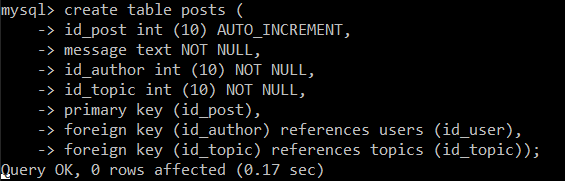
\includegraphics[width=0.6\linewidth]{images/create-posts}
	\caption{}
	\label{fig:create-posts}
\end{figure}
%\begin{lstlisting}
%create table posts (
%	id_post int (10) AUTO_INCREMENT,
%	message text NOT NULL,
%	id_author int (10) NOT NULL,
%	id_topic int (10) NOT NULL,
%	PRIMARY KEY (id_post),
%	FOREIGN KEY (id_author) REFERENCES users (id_user),
%	FOREIGN KEY (id_topic) REFERENCES topics (id_topic)
%);
%\end{lstlisting}


\end{document}




